\documentclass[11pt]{article}
\pagestyle{plain}

\usepackage{amssymb}
\usepackage{amsmath}
\usepackage{amsfonts}
\usepackage{graphics}
\usepackage{graphicx}
\usepackage[margin=1in]{geometry}
\usepackage{svg}
\usepackage{float}

\title{LINMA1170 - Devoir 2}
\author{Giovanni Karra - 45032100}

\begin{document}

\maketitle

\section*{Question 1}
Nous souhaitons étudier la sensibilité de la solution d'un problème par rapport à des perturbations dans l'entrée. Le nombre de conditionnement $\kappa$ d'un problème est la borne supérieur du ratio entre la perturbation relative de la solution et celle introduite dans l'entrée. \\
Plus formellement, si on considère une fonction $f$ comme la solution et $x$ comme l'entrée, nous avons :
\begin{align}
    \kappa = \sup_{\delta x}\left. \frac{||\delta f||}{||f||} \middle/ \frac{||\delta x||}{||x||} \right.
\end{align}
Il est important de préciser que le conditionnement s'applique uniquement les propriétés mathématiques d'un problème, et non pas la perturbation causée par un algorithme qui résout le problème (voir \textit{stabilité}).\\
Pour le problème des moindres carrées, cette borne peut être facilement calculée avec deux formules\footnote{cf Trefethen pp 129 pour la démonstration} qui donnent le nombre de conditionnement selon $A$ et selon $b$ respectivement :
\begin{align}
    \kappa_b = \frac{\kappa(A)}{\eta \cos(\theta)}~~~~~~~\kappa_A = \kappa(A) + \frac{\kappa(A)^2\tan(\theta)}{\eta}
\end{align}
avec
\begin{align}
    y = Ax ~~~ \eta = \frac{||A||||x||}{||y||} ~~~
    \theta = \arccos\left(\frac{||y||}{||b||}\right)
\end{align}
Pour vérifier cette borne numériquement, il suffit de générer des perturbations de différentes tailles, et de plotter la norme relative de la perturbation de l'entrée contre celle de la solution, comme nous pouvons le voir ci-dessous.
\begin{figure}[H]
    \centering
    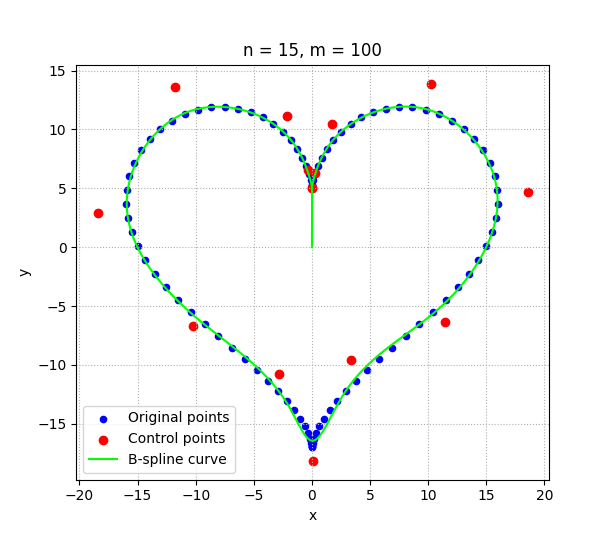
\includegraphics[scale=0.5]{../../Devoir1/rapport/images/coeur1.png}
    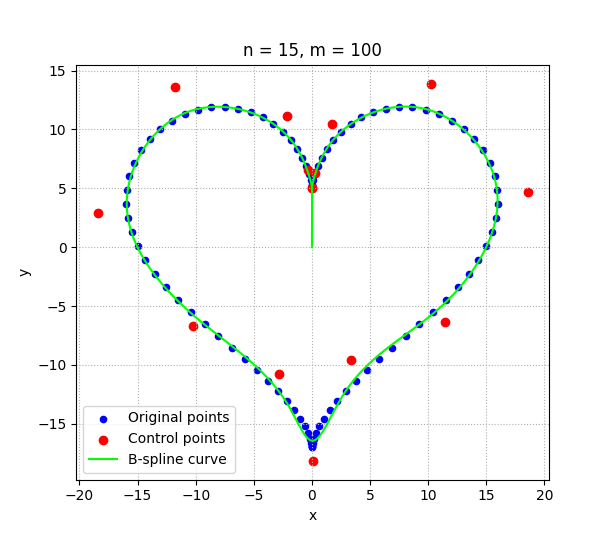
\includegraphics[scale=0.5]{../../Devoir1/rapport/images/coeur1.png}
    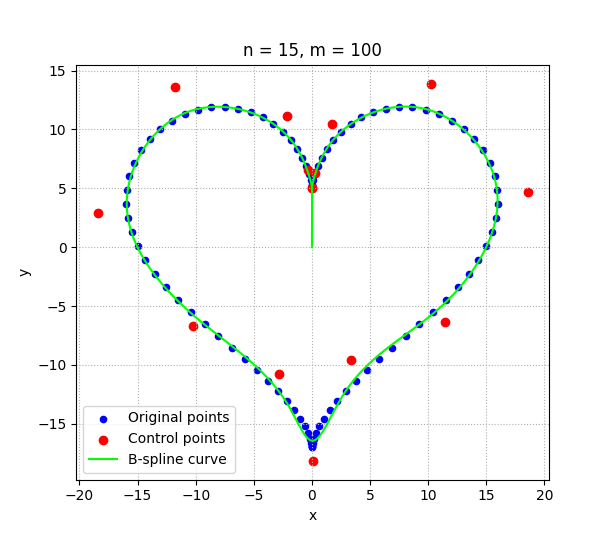
\includegraphics[scale=0.5]{../../Devoir1/rapport/images/coeur1.png}
    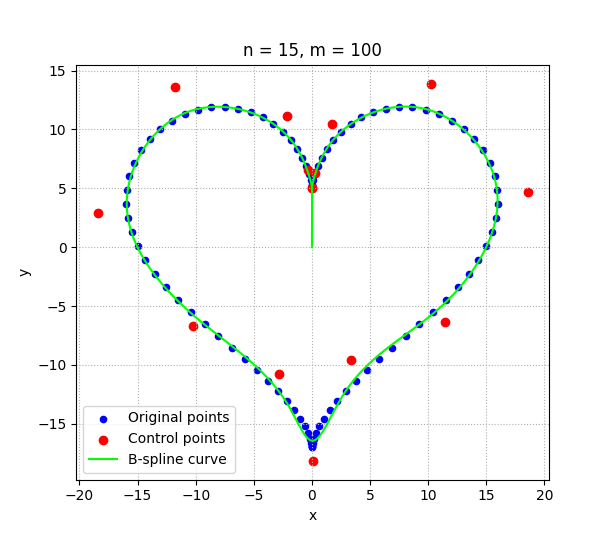
\includegraphics[scale=0.5]{../../Devoir1/rapport/images/coeur1.png}
\end{figure}
Nous pouvons voir que la perturbation empirique de la solution ne dépasse jamais la borne calculée mathématiquement.


\section*{Question 2}
La complexité temporelle de l'algorithme de décomposition $LU$ est de $\mathcal{O}(\frac{2}{3}m^3)$, $m$ étant le nombre de lignes/colonnes de la matrice carrée de départ.\\
Cet algorithme n'est pas facilement parallélisable, vu que les opérations sur les lignes dépendent des opérations réalisées sur les lignes précédentent.


\section*{Question 3}
\textit{cries in loser}


\section*{Question 4}
Résoudre un problème des moindres carrés revient à resoudre l'équation normale, c'est-à-dire résoudre le système d'équations
\begin{align}
    \tilde{A}x = \tilde{b}
\end{align}
avec
\begin{align}
    \tilde{A} = A^TA ~~~~~~~~~~~ \tilde{b} = A^Tb
\end{align}
Au lieu d'utiliser la décomposition $LU$ pour résoudre ce système, nous pouvons utiliser la factorisation de Cholesky, qui exploite la symétrie et la définie-positivité de $\tilde{A}$ pour accélérer le processus. En effet, la factorisation de Cholesky utilise en théorie deux fois moins d'opérations que la décomposition $LU$, et nous pouvons vérifier ceci empiriquement sur les figures ci-dessous.
\begin{figure}[H]
    \centering
    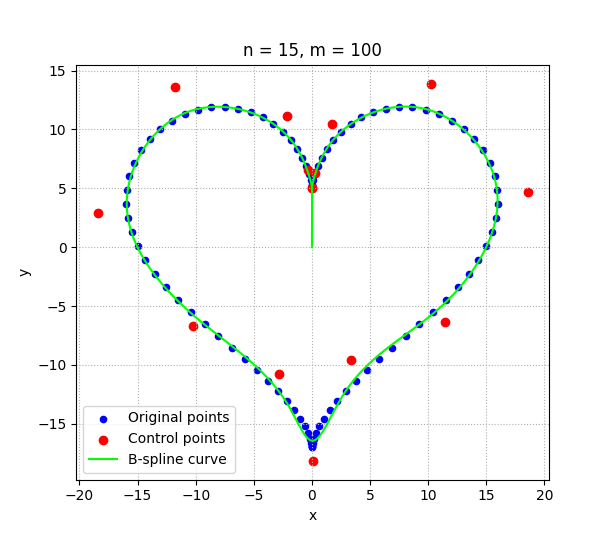
\includegraphics[scale=0.5]{../../Devoir1/rapport/images/coeur1.png}
    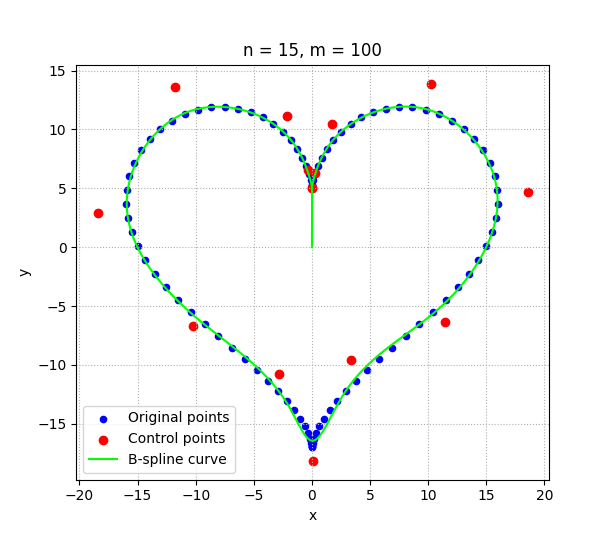
\includegraphics[scale=0.5]{../../Devoir1/rapport/images/coeur1.png}
\end{figure}

\end{document}